%!TEX root = ../main.tex
\chapter {Wegweiser zu den wichtigsten Latexstrukturen}\label{text:main}

\section {Tabellen}

Damit man sich die Einbettung der Tabelle im Text besser vorstellen kann, steht hier ein wenig Text. Eine Tabelle könnte folgendermaßen aussehen:

	\begin{table}[h]
		\begin{center} %Zum zentrieren der Tabelle, sieht meistens besser aus, weil die Tabellenüberschrift immer zentriert wird...
			\caption[Kurzfassung f. Inhaltsverz.]{So könnte eine Beispieltabelle aussehen} \vspace{2ex} %Die Caption ist die Tabellenunterschrift
			
			\begin{tabular}{lll}        % Die Tabelle soll drei linksbündige Spalten enthalten, 
										% alternativ r für rechtsbündig und c für zentriert, 
										% ein | fügt einen vertikalen Trennstich ein
	        \hline                      %  horizontale linie
			\textbf{Fahrzeugtyp} & \textbf{Hersteller}& \textbf{Modell}\\
			\hline                      % horizontalen Linien 
			  &\\
			  Sportwagen & Porsche & 911 GT2 \\
			   & Ferrari & Enzo \\
			  Kleinwagen & Volkswagen & Polo \\
			   & & Lupo \\
			  Familienwagen & Ford & Mondeo \\
			   & BMW & 525d \\
			  \hline
			 \end{tabular}
			\label{tbl:Autos}		% Das Label dient zum Referenzieren im Dokument
		\end{center}
	\end{table}

Unter der Tabelle geht es dann weiter mit dem Text. Es gibt auch noch andere Möglichkeiten für Tabellen. Zum Bespiel kann man Zellen zusammenfassen:

Komplexere Beispieltabelle unter Benutzung des array-Packages:


Eine Tabelle mit dem booktabs-style (Die zwei folgenden Beispiel stammen aus dem Internet\linebreak (\url{http://www.unix-ag.uni-kl.de/~fischer/blog/20070411_Tabellen_in_LaTeX/}), ich hatte keine Lust mir einen neuen Text auszudenken und die Lösung für das Multirow-Problem wollte ich auch nicht neu erfinden)\\[1.5ex] %Zeilenumbruch mit zusätzlichem Abstand (1.5 mal die Höhe des Buchstaben x)
Dann sieht die Tabelle wie folgt aus:
	
	\begin{table}[H] % Achtung: Mit diesem Befehl erzeugt man ein float-Objekt, also etwas, was von LaTeX automatisch dort platziert wird, wo es am besten aussieht, 
								% das ist nicht immer der Ort, wo man sie auch haben möchte. Abhilfe schafft z.B. das Package float und die Platzierungsoption "H". Also: \begin{table}[H]
		\caption[Schöne Tabelle]	{Das ist eine schöne Tabelle. Damit die Tabelle, wie allgemein üblich eine Überschrift und keine Unterschrift bekommt, 
															 muss der \emph{caption}-Befehl oberhalb der Tabellenbefehle, aber innerhalb der \emph{table}-Umgebung stehen. 
															 Schreibt man den \emph{caption}-Befehl unterhalb der \emph{tabular}-Umgebung, so erscheint auch einen \underline{Unter}schrift 
															 (wie bei Abbildungen üblich)}
		\begin{center} % Achtung: Dieser Befehl erzeugt zusätzlich zu dem zentrieren auch noch einen zusätzlichen vertikalen Abstand.
			\begin{tabular}{lll}
				\toprule
					Author & Title & Year 
				\\ \midrule
					\multirow{3}{*}{Philip K. Dick} & Minority Report & 1956 
				\\ \cmidrule{2-3}
		 			& Do Androids Dream of Electric Sheep? & 1968 
				\\ \cmidrule{2-3}
		 			& A Scanner Darkly & 1977 
				\\ \midrule
					\multirow{3}{*}{Neal Stephenson} & Snow Crash & 1992 
				\\ \cmidrule{2-3}
		 			& The Diamond Age & 1995
				\\ \cmidrule{2-3}
		 			& Cryptonomicon & 1999
				\\ \bottomrule\\
			\end{tabular}
		\end{center}
	\end{table} 
	
	Tabellen bei denen sich in einigen Spalten Text und in anderen Spalten Matheformeln befinden, definiert man am besten unter Benutzung des array-Paketes. Hier lässt sich am Anfang bzw. Ende einer Zelle ein beliebiger Text einfügen. das funktioniert mit ,,>\{Text\}'' bzw. ,,<\{Text\}''. Statt einem Text kann man nun einfach jeweils ein \$ einfügen und hat so eine Mathe-Spalte. Wenn man immer zwischen zwei Spalten einen bestimmten Text wie z.B. ein ,,='' haben will, kann man das durch ,,\@\{=\} erhalten. Verschönerungen wie zusätzliche Abstände etc. kann man ebenfalls einplanen. 
	
	Hier noch ein einfaches Beispiel:
	
\begin{center}
	{\centering % der Centering-Befehl erzeugt keinen zusätzlichen vertikalen Abstand.  Der Befehl und die zu zentrierenden Objekte müssen in geschweifte Klammern...
		\begin{tabular}{l>{$}c<{$} @{\;$=$\;}>{$}c<{$}}
		\toprule
		Formel 1 & \alpha & 7\cdot \beta
		\\ \midrule
		Formel 2 & x^2 & \alpha + \beta
		\\
		& & 8\cdot \alpha
		\\ \bottomrule
		\end{tabular}
	}
\end{center}

\textbf{HINWEIS:} Ein sehr hilfreiches Tool zum Erstellen von Exceltabellen ist das Excel-Plugin \glqq Excel2Latex\grqq. Damit lassen sich Tabellen sehr einfach von Excel in den Latex-Code transferieren.


\section{Mathematische Formeln}

Einzelne Formeln werden über eine \emph{Equation}umgebung
eingebunden

\begin{equation}\label{eqn:Testgleichung}
    \alpha = \beta \cdot \gamma + \delta
\end{equation}

% % Achtung: Die Eqnarray-Umgebung ist veraltet und sollte nicht mehr verwendet werden!
%Während mehrere Formeln über eine \emph{eqnarray}-Umgebung 
%übersichtlich ausgerichtet werden können.
%\begin{eqnarray}
%% \nonumber to remove numbering (before each equation)
%  \delta &=& \alpha - \beta \cdot \gamma \nonumber \\
%  \gamma &=& \frac{\alpha - \delta}{\beta}\label{eqn:Testgleichungsarray}
%\end{eqnarray}
Mehrere Formeln können mit der \emph{align}-Umgebung ausgerichtet werden:
	\begin{align}
		\delta &= \alpha - \beta \cdot \gamma & d &= f+q
		\nonumber 
			% use \nonumber or \notag to remove numbering; 
			% use \tag{OwnTag} to create a personal tag or \tag*{} to create tag without parantheses (works also in nonumbered environment)
	  \\
	  \gamma &= \frac{\alpha - \delta}{\beta}
	  \label{eqn:Testgleichungsarray}
	\end{align}

Die Nummerierung in den \emph{equation}- und \emph{align}-Umgebungen kann durch \emph{equation*} bzw. \emph{align*} unterdrückt werden.

In Gleichung~\ref{eqn:Testgleichungsarray} kann man sehen, wie man mit der \emph{align}-Umgebung Formeln anordnen kann. Grundsätzlich werden, wie bei
Abbildungen und Tabellen auch Formeln durchnummeriert. Wenn das nicht gewünscht ist, also z.B. im obigen Gleichungsarray, die
zweite Gleichung nur eine Umformung der ersten ist, reicht ein \emph{$\backslash$nonumber} vor dem Umbruch \emph{$\backslash\backslash$} um eine Nummerierung zu
unterdrücken. Wenn man die gesamte Nummerierung unterdrücken möchte, fügt man dem Befehl einfach ein * hinzu, man verwendet also z.B. $\backslash$begin$\{$align*$\}$.
Abgesetzte Formeln ohne Nummerierung können auch mit den Befehlen \textbackslash [ und \textbackslash ] erzeugt werden. 

Selbstverständlich können auch im laufenden Text Formeln wie
$\cos^{2}{x}+\sin^{2}{x}=1$ eingebunden werden.

Einheiten werden in Mathematikumgebungen mit
\emph{$\backslash$mathrm} im Gegensatz zur restlichen Formel und
Formelzeichen \textbf{nicht} kursiv dargestellt:

\begin{eqnarray}
% \nonumber to remove numbering (before each equation)
  l * b &=& A \\
  5 \mathrm{m} \cdot 2 \mathrm{m} &=& 10 \mathrm{m^{2}}
\end{eqnarray}

\section{Chemische Formeln}

	Um chemische Formeln sinnvoll zu setzen gibt es das Paket \emph{mhchem}. Dieses Paket stellt die für chemische Reaktionen nötigen Reaktionspfeile zur Verfügung 
	und setzt chemische Formeln in nicht kursiven Buchstaben.
	
	Das mhchem-Paket kann chemische Formeln wie dieses hier \ce{|\nu_A|\, A + |\nu_B|\, B <=>[oben][unten] |\nu_P|\, P + |\nu_Q|\, Q} in den Text einbinden. 
	Die Gleichungen werden am Zeilenende umgebrochen, das ist nicht immer schön. 
	
	Außerdem kann man die Befehle auch im Mathemodus einbinden und so die Gleichungen mit durchnummerieren. 
		\begin{equation}
			\ce{|\nu_A|\, A + |\nu_B|\, B <=>[oben][unten] |\nu_P|\, P + |\nu_Q|\, Q}
		\end{equation}
	
	Weitere Möglichkeiten zu dem Package findet man in der ausführlichen Dokumentation.
	
	Wenn man organische Moleküle in ihrer Struktur zeichnen will, bietet sich das Package \emph{chemfig} an. Die etwas komplizierte Benennung der Winkel entnimmt man am besten wieder der Dokumentation. Im Folgenden zwei Beispiel:
	\subsection{Trifluoroessigsäure (TFA)}
		
			Formel:\quad \ce{C2HF3O2}
			\hspace*{3em}
			\chemfig{C(-[2]F)(-[4]F)(-[6]F)-C(-[1]OH)=[7]O}
			\hspace*{3em}
			\chemfig{(-[3]F)(<:[:-150]F)(<[:-100]F)-(-[1]OH)=[7]O}\\[2ex]
			
		\subsection{Dichlormethan (DCM)}
			
			Formel:\quad \ce{CH2Cl2} 
			\hspace*{5em}
			\chemfig{C(-[5]Cl)(-[2]Cl)(<[:-70]H)(<:[:-20]H)}\\[2ex]
			

\section{Bilder}

Bilder werden mit Hilfe der ''figure''-Umgebung eingebunden. Dabei
kann die Breite festgelegt werden. Es empfiehlt sich, hier keine
absoluten Werte in Zentimetern anzugeben, sondern Bezug auf die
Textbreite zu nehmen. Das folgende Bild wurde mit 30 Prozent der
Textbreite eingebunden, \emph{0.3$\backslash$textwidth}. Alternativ kann man die Größenangeabe weglassen und das Bild in Originalgröße einbinden, die Texthöhe (textheight) oder cm-Angaben verwenden.


	\begin{figure}[h!bt]	% Requires \usepackage{graphicx}
		\begin{center}
		  \includegraphics[width=\textwidth]{rwth_avt_rgb}
		  \caption{Testbild}\label{fig:Testbild}
		\end{center}
	\end{figure}

 \begin{figure}[H]
    \centering
        \begin{subfigure}[t]{0.45\textwidth}
            \centering
            \includegraphics[width=\textwidth]{4_images/Beispiel-Graph.png}
            \caption{}
            \label{subfig:graph1}
        \end{subfigure}
        \hfill
        \begin{subfigure}[t]{0.45\textwidth}
            \centering
            \includegraphics[width=\textwidth]{4_images/Beispiel-Graph.png}
            \caption{}
            \label{subfig:graph2}
        \end{subfigure}
    \caption{Graphen für Ergebnisse werden mit Origin erstellt. Ein Tutorial kann unter https://cvtwiki.avt.rwth-aachen.de/wiki/doku.php?id=sop:data\_management:origin gefunden werden. Achtung, der Link lässt sich nur aus der pdf öffnen, wegen des \_.}
    \label{fig:graphs}
\end{figure}


Mögliche Bildformate sind *.jpg, *.png, *.gif, *.pdf.

Das Einbinden von Bildern erfolgt mit der  $\backslash begin\{ figure\}...\backslash end\{ figure\}$-Umgebung als sogenanntes Float-Element, mit dem die Position von Latex selber angepasst werden kann. Die Option [H] zwingt das Float-Element genau an die stelle im Text an der das Element im Quelltext eingebunden wurde.

\section{Fußnoten}
Ein kurzer Beispieltext mit Fußnoten:

Grundsätzlich gilt: Ein Blick in die Literatur spart viel mehr
Zeit als sie kostet! Und damit sie noch weniger Zeit kostet, sind
die wichtigsten Wege zur Recherche und Beschaffung von Literatur
an der RWTH im AVT-Wiki\footnote{Wikis haben den Vorteil das sie
kontinuierlich verbessert werden können, während dieses Dokument
doch eher statischer Natur ist} zusammengestellt. Die angegeben
Informationsquellen stellen nur eine Übersicht über die
Möglichkeiten dar und haben nicht den Anspruch auf
Vollständigkeit, können aber mit Hilfe aller Nutzer diesen Zustand
anstreben. Zu finden ist der Wegweiser zur Literaturbeschaffung
auf
\url{https://wiki.avt.rwth-aachen.de}
zu finden.\footnote{Diese URL ist nur an Institutsrechnern oder
über den entsprechenden Login erreichbar}

\section{Graphen und Zeichnungen}

Graphen können ohne viel Aufwand mit PGFplots erstellt werden. Beispiele gibt es unter \url{http://pgfplots.sourceforge.net/gallery.html}.
\begin{center}
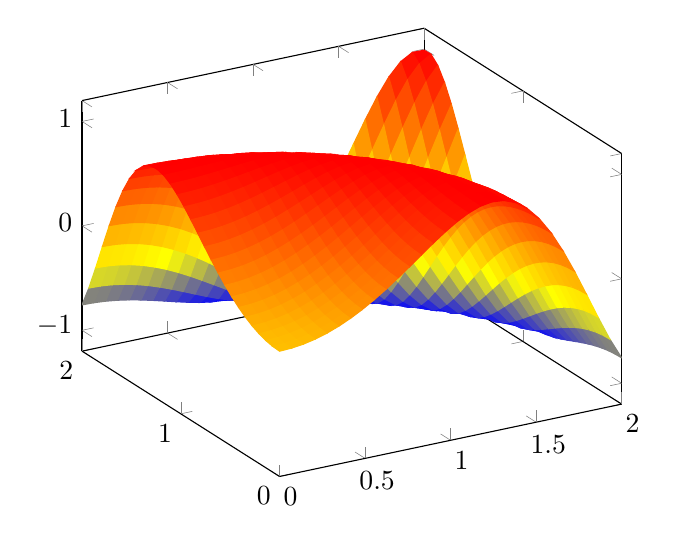
\begin{tikzpicture}
	\begin{axis}[view/h=-30]
	\addplot3[
		surf,
		shader=flat,
		samples=30,
		domain=0:2,y domain=0:2] 
		{sin(deg(x^2+y^2))};
	\end{axis}
\end{tikzpicture}
\end{center}

Zeichnungen können unkompliziert mit Tikz angefertigt werden. Siehe \url{http://www.texample.net/tikz/examples/}.
\begin{center}
\begin{tikzpicture}[->,>=stealth',shorten >=1pt,auto,node distance=4cm,semithick]
  \node[state] (A){$s_0$};
  \node[state] (B) [above right of=A] {$s_1$};
  \node[state] (C) [below right of=B] {$s_2$};

  \path 
    (A) edge [bend left] node{0,2}(B)
        edge node {0,2}(C)
    edge [loop left] node{0,6}(A)
    (B) edge [loop above] node{0,5}(B)
        edge [bend left] node{0,4}(C)
    edge node{0,1}(A)
    (C) edge node{0,2}(B)
        edge[bend left] node{0,3}(A)
    edge[loop right] node{0,5}(C);
\end{tikzpicture}
\end{center}


\section{Internetadressen}

Abhilfe bei (fast) allen Problemen bietet der Befehl \emph{url}:

\url{https://avt.rwth-aachen.de}

Dann sollte ein Zeilenumbruch erfolgen. Achtung, auch hier gibt es ein Sonderzeichen, das Probleme machen kann und das ist das \%, da man damit in \LaTeX\ den Rest der Zeile auskommentiert. Hier muss man wieder \textbackslash \% schreiben.

\section {Listen}
Hier sei zunächst auf einige nützliche Zusammenstellungen von
Stoffdaten verwiesen, um das Einfügen einer unnummerierten Liste
zu demonstrieren:
\begin{itemize}
    \item Eine sehr gute Übersicht findet man auf den Seiten des \emph{\textbf{National Institute of Standards and Technology}} (www.nist.gov) unter Information for Researchers.
    \item \emph{\textbf{Perry's Chemical Engineers' Handbook}}, Kapitel 2 (IVT-Bibliothek)
    \item \emph{\textbf{CRC Handbook of Chemistry and Physics}} (IVT-Bibliothek)
    \item \emph{\textbf{Handbook of Electrolyte Solutions}} (zweibändig, unter Signatur E7146 im Großen Lesesaal der HSB)
    \item \emph{\textbf{Gmehling-Onken}}, Sammlung Thermochemischer Stoffdaten, vor allem Gas-Flüssig Gleichgewichte (mehrbändig, unter Signatur E0218 im Großen Lesesaal der HSB sowie in der Bibliothek der AVT.TVT)
    \item In der Chemiebibliothek in der Prof.-Pirlet-Str. finden sich weitere Material- und Datensammlungen. Das Stöbern lohnt sich.
    \item Im Programmpaket \emph{\textbf{ASPEN Plus}} ist eine umfangreiche Stoffdatenbank integriert, die auch unabhängig von einer Prozesssimulation abgefragt werden kann.
    \item   \begin{enumerate}
        \item \textbf{Selbstverständlich können Listen auch geschachtelt
        werden}
        \item Nummerierte Listen sind auch möglich, nur heißt dann die Umgebung nicht ''itemize'' sondern ''enumerate''
            \end{enumerate}

\end{itemize}

		\section {Gliederung}
			Wichtig ist nicht nur die technisch richtige Gliederung in Tex,
			sondern auch das richtige bezeichnen in der Arbeit. So heißt
			dieses Kapitel ''Wegweiser zu den wichtigsten Latexstrukturen''
			und sollte auch so benannt werden.
			
			Ist das Unterkapitel ''Gliederung'' gemeint, sollte es bei
			Verweisen auch so genannt werden. Gleiches gilt für
			\subsection {Abschnitte}
			Abschnitte
			\subsubsection {Unterabschnitte}
			Unterabschnitte und
			\paragraph {Absätze}
			Absätze
			
			Diese Gliederungseinheiten können übrigens auch im Code mit einem
			* hinter dem Namen versehen werden. Dann wird eine Nummerierung
			unterdrückt und die Überschrift nicht im Inhaltsverzeichnis
			gelistet. Sinn macht das aber nur bei Kapiteln, Unterkapiteln und
			Abschnitten, da nur diese nummeriert werden.

		\section {Umgebungen}
			Tabellen, Bilder und Gleichungen werden in Latex in der Regel in
			Umgebungen geschrieben. Bei Tabellen und Bildern enthalten diese
			oft den \textbf{$\backslash$caption$[x]$\{y\}}-Befehl. y steht in
			diesem Fall für die Bild-/Tabellen Unter- bzw. Überschrift,
			abhängig davon, ob der Befehl in der Umgebung vor oder nach dem
			Objekt
			steht.\\
			x ist optional und steht für eine Kurzbeschreibung, falls y zu
			lang für das Abbildungs- oder Tabellenverzeichnis ist.
			
			\subsection {Referenzen}
			Um auf bestimmte Textstellen oder Objekte zu verweisen, bedient
			man sich in Latex sogenannter Labels und Referenzen. Ein Label
			wird mit dem Befehl \textbf{$\backslash$label\{name\}} gesetzt.
			Der Name sollte hier möglichst intuitiv gesetzt werden. Es ist
			sinnvoll hier auch den Typ des verwiesenen Objektes einzubeziehen,
			z.B. ist es empfehlenswert den Namen bei Gleichungen mit ''eqn:''
			zu beginnen, bei Bildern mit ''fig:'' und bei Tabellen mit
			''tab:''.
			
			Sehr wichtig ist, dass bei Bildern und Tabellen die
			\textbackslash label-Anweisung unmittelbar auf die
			\textbackslash caption-Anweisung und bei Gleichungen noch in derselben Zeile steht, da sonst auf die Textstelle statt auf das
			Objekt verwiesen wird.
			
			Neben den nummerierten Referenzen mit \textbf{$\backslash$ref\{name\}}, wie z.B. auf Gleichung
			\ref{eqn:Testgleichungsarray}, ist mit \textbf{$\backslash$pageref\{name\}} der Hinweis möglich, dass
			besagte Gleichung auf Seite \pageref{eqn:Testgleichungsarray} zu finden ist. Besonders interessant ist 
			der Befehl \textbf{\textbackslash eqref\{name\}} für mathematische Gleichungen, da hier automatisch die Klammern um die
			Referenznummer mitgesetzt werden.
			
		
		\section {Hinweise zum Literaturverzeichnis}
			
			Die für das Literaturverzeichnis verwendeten Daten, werden in einem externen file mit der Endung .bib gespeichert. Diese Datei kann theoretisch in jedem Texteditor erstellt und bearbeitet werden, solange man sich an die vorgegebene Syntax hält. 
			Einfacher ist die Verwendung des Open Source Tool \emph{JabRef}, das eine Maske mit Feldern bereitstellt, bei denen auch vorgegeben ist, welche Angaben benötigt werden und welche nicht unbedingt. Außerdem kann man in JabRef auch Zusatzinformationen wie den Abstract der Paper speichern und die Literatur verwalten.
			
			Das zitieren erfolgt über den sogenannten Bibtex-Key mit dem Befehl \textbackslash cite\{BibtexKey\}. Das Literaturverzeichnis wird automatisch nach \textbf{zweimaligem} kompilieren aktuell erstellt (Beim ersten Kompilieren werden die Daten der .bib-Datei ausgelesen und beim zweiten Kompilieren wirklich verknüpft). 
			
			
			Und so sieht das dann praktisch aus: Das hier ist eine sehr interessante Quelle \cite{Abel2000}, man sollte aber auch dieses Paper unbedingt gelesen haben \cite{Marquardt2005}. Dabei ist die autovervollständigen Funktion vom TeXnicCenter durchaus hilfreich. Wenn man einen der Befehle \textbackslash cite oder \textbackslash ref verwendet, bekommt man nach dem Tippen der ersten Zeichen des Keys Vorschläge, die man mit Strg + Leertaste annehmen kann.


		